%%%%%%%%%%%%%%%%%%%%%%%%%%%%%%%%%%%%%%%%%%%%%%%%%%%%%%%%%%%%%%%%%%%%
%
% IMPERIAL COLLEGE LONDON DISSERTATION TEMPLATE 
%
%%%%%%%%%%%%%%%%%%%%%%%%%%%%%%%%%%%%%%%%%%%%%%%%%%%%%%%%%%%%%%%%%%%%
%
% This file is `icldiss.tex'
%
% This document fulfills the layout requirements for Dissertations
% of the University of London and of Imperial College London.
% To do so it uses the documentclass `icldt' which is provided free 
% of charge under the MIT license. The relevant College regulations,
% and the license are included in the `icldt' manual.
%
% If you print your dissertation for yourself or as a present for
% family, friends or colleagues you probably should use a different
% layout which does not fulfill the College requirements but which
% can look much better.
%
% For further information and for professional layouting and
% printing services please visit www.PrettyPrinting.net
%
% Copyright (c) 2008, Daniel Wagner, www.PrettyPrinting.net
%
%%%%%%%%%%%%%%%%%%%%%%%%%%%%%%%%%%%%%%%%%%%%%%%%%%%%%%%%%%%%%%%%%%%%

\documentclass[MSc]{icldt}

\usepackage{parskip}
\usepackage[latin1]{inputenc}
\usepackage{tikz}
\usetikzlibrary{shapes,arrows}
\usepackage{float}
\usepackage{listings}
\usepackage{color}

\definecolor{dkgreen}{rgb}{0,0.6,0}
\definecolor{gray}{rgb}{0.5,0.5,0.5}
\definecolor{mauve}{rgb}{0.58,0,0.82}

\lstset{frame=tb,
  language=Java,
  aboveskip=3mm,
  belowskip=3mm,
  showstringspaces=false,
  columns=flexible,
  basicstyle={\small\ttfamily},
  numbers=none,
  numberstyle=\tiny\color{gray},
  keywordstyle=\color{blue},
  commentstyle=\color{dkgreen},
  stringstyle=\color{mauve},
  breaklines=true,
  breakatwhitespace=true
  tabsize=3
}

\title{Tree of Life Visualisation \\ By}
\author{Kai Zhong(kz12)}


% Please specify you department here.
\department{Computing}

% The college regulations do not require that you mention 
% your supervisor on the titlepage of you dissertation.
% If you want to do so put her name here.
\supervisor{}
% The college regulations do neither require nor forbid 
% a dedication of your dissertation to somebody or something. 
% If you want to include a dedication put the text here. 
\dedication{}

\date{September 2013}

\begin{document}

\maketitle

\tikzstyle{decision} = [diamond, draw, fill=blue!20, 
    text width=4.5em, text badly centered, node distance=3cm, inner sep=0pt]
\tikzstyle{block} = [rectangle, draw, fill=blue!20, 
    text width=8em, text centered, rounded corners, minimum height=4em]
\tikzstyle{line} = [draw, -latex']
\tikzstyle{cloud} = [draw, ellipse,fill=red!20, node distance=3cm,
    minimum height=2em]
    
\begin{abstract}

The storage, searching and visualisation of big data has become an increasingly important issue in computer science. One of the technique for visualisation of huge hierarchies is the interactive fractal inspired graph(IFIG), which employs fractal geometry to place limitless amounts of information on a single page and show, hide information by the simple actions of zooming and panning. This method is created by Imperial College academic Dr. James Rosindell, who has also employed it for tree of life visualisation where it solved a significant outstanding problem in evolutionary biology: how can large evolutionary trees be visualised effectively for science, education and public outreach.

While the software written by Dr. James Rosindell runs on javascript and html5, my main task is to develop an android application based on his code. Compared with personal computer, the calculation ability of a mobile device is relatively low and the RAM capability is more restricted. The project involves how to use multiple thread and temporary bitmaps to solve performance issue, which greatly shorten the loading time as well as the response time of user interaction. When dealing with larger trees, because of the limitation of RAM capability, dynamical loading and freeing objects is employed in this project, such that the usage of RAM could be maintained under the limitation of an android application. 
Both the technique of multiple thread and using dynamical loading and freeing objects could be employed in the website software.

\end{abstract}

\makededication

\tableofcontents
\listoftables
\listoffigures

\chapter{Introduction}

\section{Background}

Visualising phylogenies is one of the fundamental tasks of evolutionary analysis. It has long been a great challenge to display huge trees. When the amount of species on the tree increases to millions, no screen of paper is huge enough to display the whole tree while maintaining all details(e.g., name, population stability, conservation status) of each species. Even a screen large enough is accessible, it is unpleasant for users to look for information on such a large screen. 

One way to solve this issue is interactive fractal-inspired graph(IFIG), which concludes all species as well as all their information displaying in screen. The key concept of the IFIG method is to place all the data on one page such that users could navigate between different scales by simply zoom(http://www.onezoom.org). Therefore, users can't see all information of all species at one time. Instead, when the scale is big enough, users could see the whole picture of the tree of life but with few details of each species. When users zoom the tree, more details of the selected area will be displayed while other species might go out of the screen.

The interface of the OneZoom is analogous to Google Earth. When using google earth, one can find a location by zoom in from a start page of the whole globe, recognizing familiar landmarks at different scales along the way(e.g., continents, countries, regions, and towns)(TODO: add reference). Equivalently, OneZoom enables user zoom smoothly to the species they want to find. For example, one can find human beings by zooming in along the clades of animals, vertebrates, mammals and primates.(reference) The hierarchy dataset is represented by using fractals. Fractals are typically self similar patterns, where self similar means they are "the same from near as from far". This means the shapes of branches and nodes remains similar at different scales of zoom.(TODO: add reference) Hence, it could ensure the amount of visual elements on a screen remains relatively constant. Moreover, fractals simplify the representation of huge hierarchy dataset. All levels of data is represented in the same way. So inserting or deleting data can be automatically adopted by the software in the tree representation.

\section{OneZoom Android Application}

The IFIG method was only implemented using javascript and html5. The aim of this project is to develop an android application of it. The application is based on the javascript code written by my tutor Dr. James Rosindell. 

When the application was developed, the first issue came to me is that the loading time of a tree is over long. This problem also occurs in the website software, though it is not very obvious due to faster processor of personal computer than mobile device. The fluency of user interaction is another issue. There were apparent delays when users interacted with the application. Both of this issues has been solved and details of that will be discussed in Chapter 4.

As the data gets larger, more memory needs to be allocated. As the memory one android application could be allocated is quite small, the application sometimes got crashed when drawn the tree of tetrapods which has over 22 thousand species. This is also a potential issue for the further development of the software on OneZoom website when the size of tree grows to over million species. A more detail description of this problem the solution of it will be discussed in Chapter 5.



\section{Structure of this Report}

Chapter 2 gives introduction to the software that I am going to build on. It includes what interactions could users have with this software, the basic structure of the software, what methods are used to increase the performance of the software as well as some functions that I would inherited in the mobile application. Chapter 3 mainly talks about some changes in the implementation of the node class and how the application listens user interactions. 

Chapter 4 discusses ways to improve the performance of the application. It includes shortening loading time as well as making user interaction more fluent. When dataset gets larger, the application will hit memory limitation. Chapter 5 gives a description of this issue and also the solution for it.

Chapter 6 goes through other functionalities that the application has implemented.
 

\chapter{OneZoom Website Software Introduction}

In this chapter, I would like to give a brief introduction to the OneZoom website software code, which was given by Dr. James Rosindell and my whole project has been built on it. This software is accessible on the official website for this project: www.onezoom.org. 

\section{How to use the software}
Basically, the OneZoom software allows users to explore the tree of life in a completely new way: it's like a map, everything is on one page, all you have to do is zoom in and out(reference). When a user zooms in, some nodes become visible and more details will be shown on nodes. On the other hands, when a user zooms out, some nodes become invisible and some details will disappear in order to provide user a neat view. 

For example, in the figure of the tree of mammal, the tail of the tree is covered by a signpost rodents. If we zoom in this area, we can see that more signposts appears telling us more details of the rodent family. If we continue zoom in the mouse-like rodents, we can see that nodes that was invisible in the first two figures emerging.

\begin{figure}[H]
  \centering
  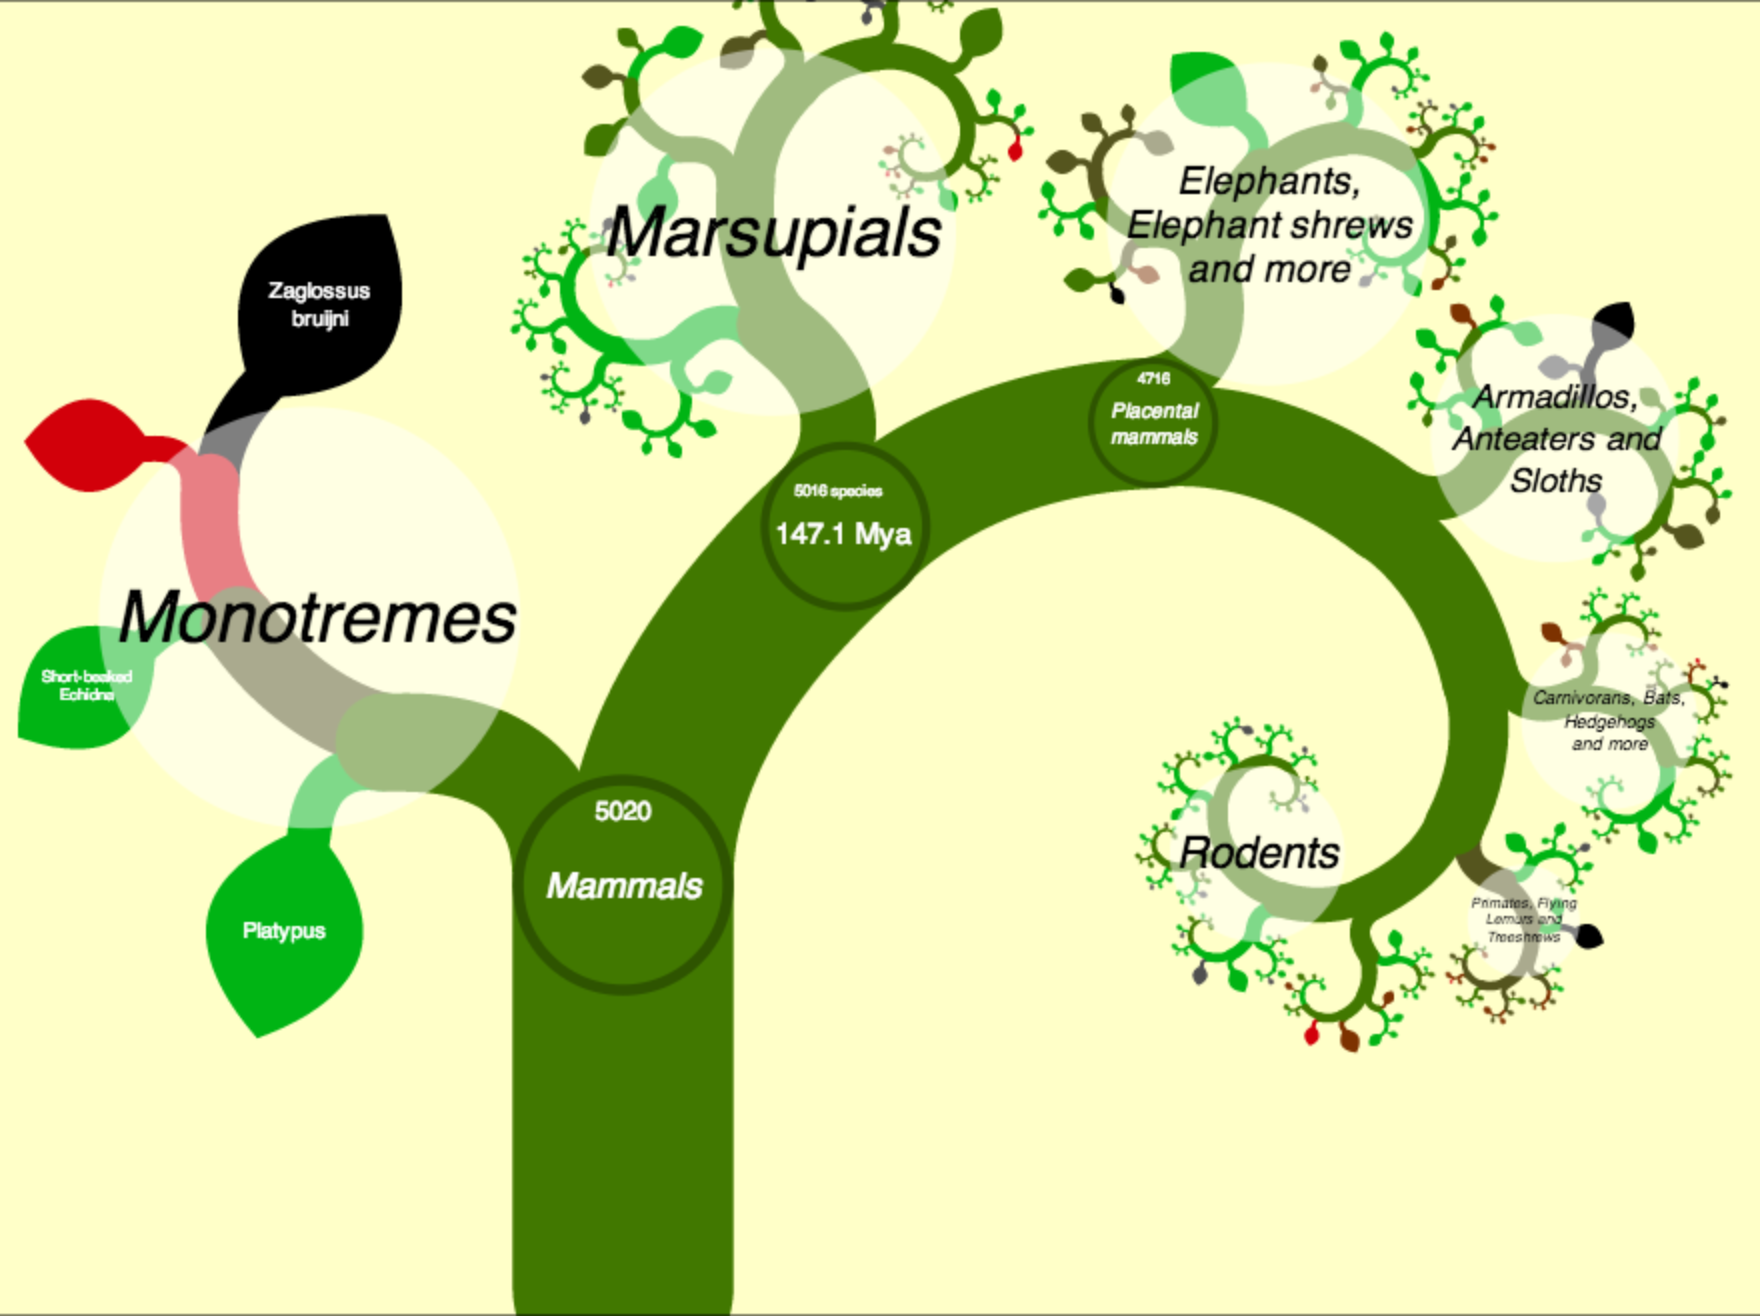
\includegraphics [width=15cm,height=8.8cm]{Mammal}
  \caption{Tree of Mammal}
  \label{fig:mammal}
\end{figure}

\begin{figure}[H]
  \centering
  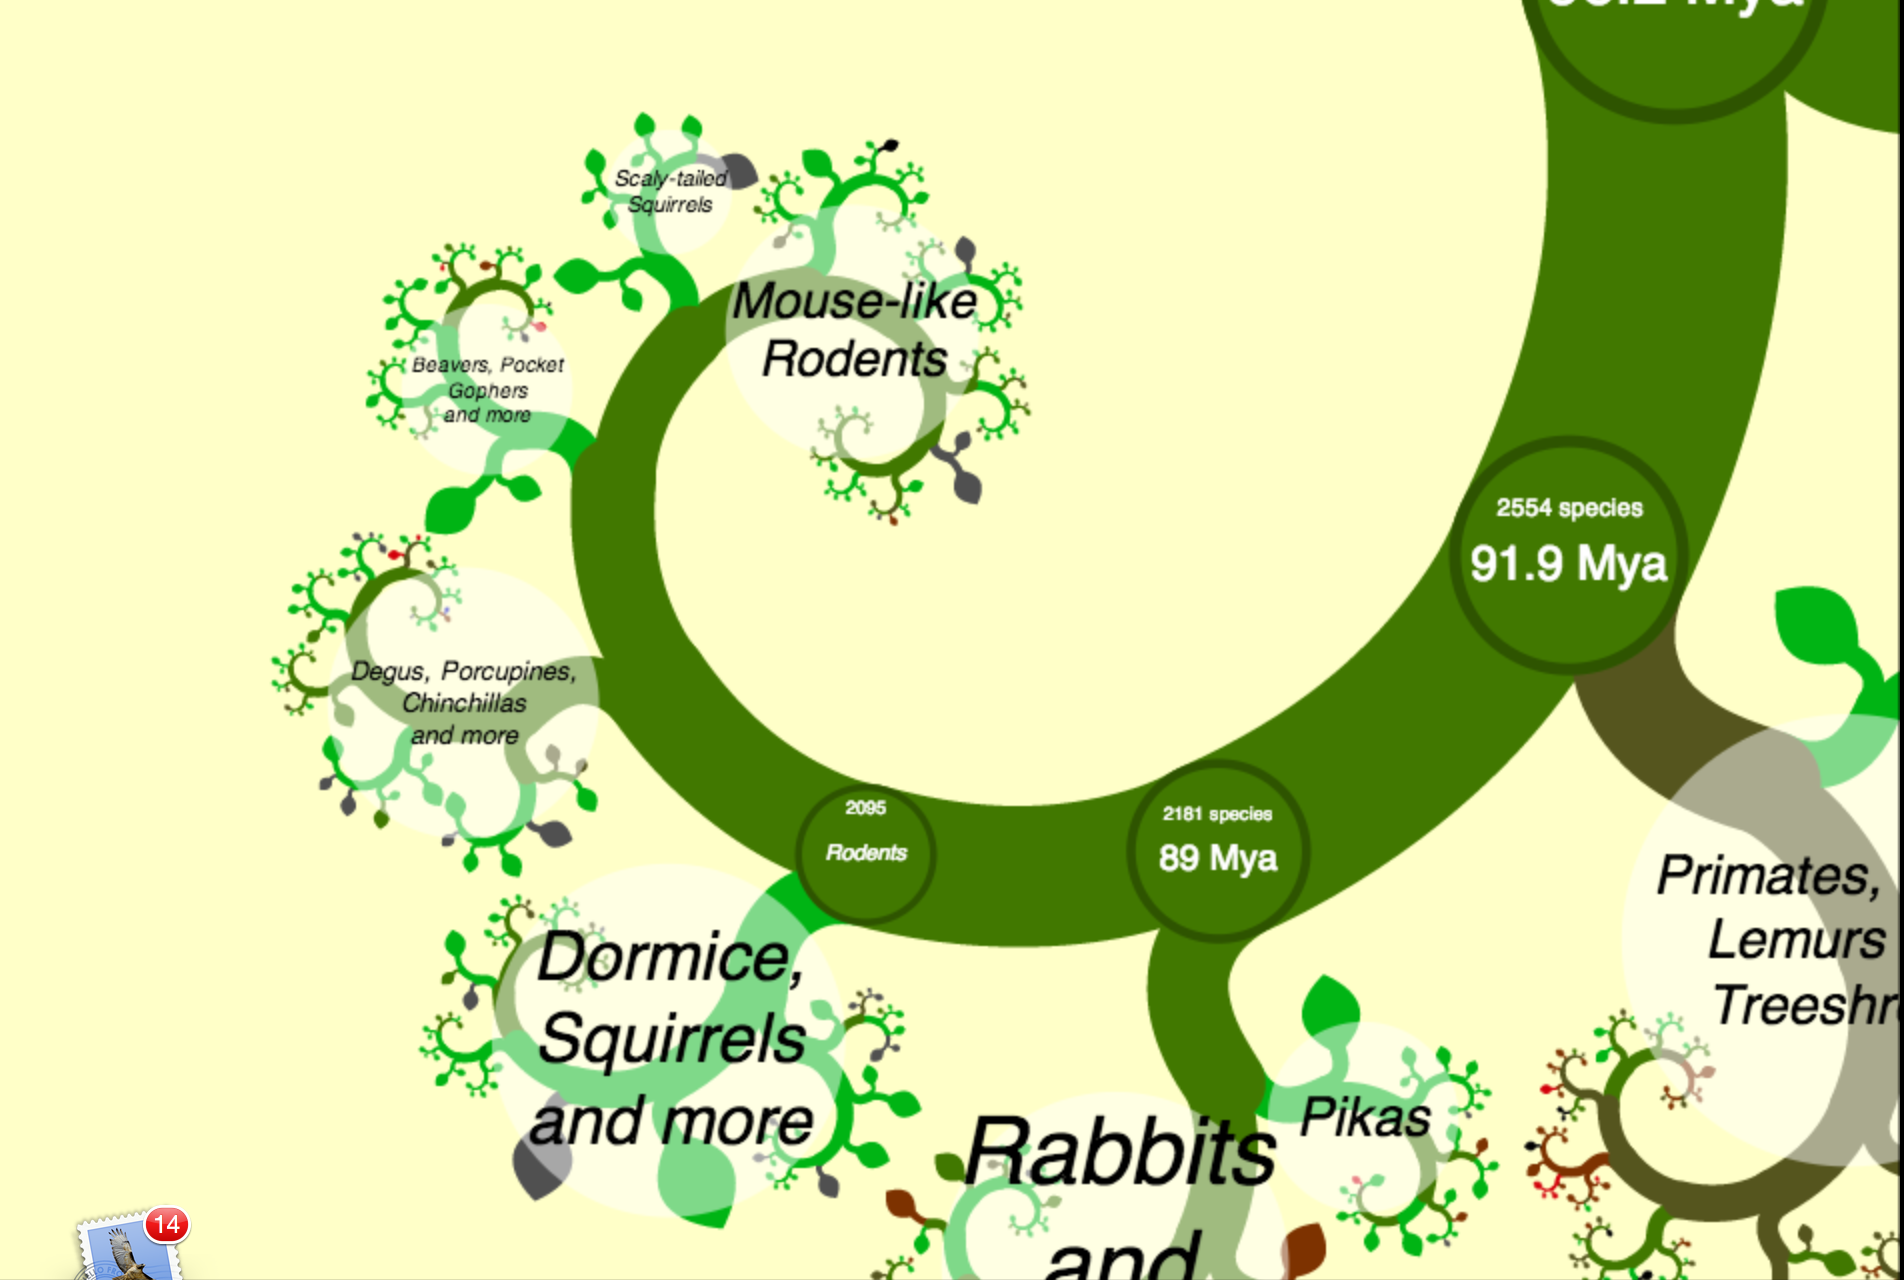
\includegraphics [width=15cm,height=8.8cm]{Rodent}
  \caption{Tree of Rodent: Zoom In the Rodent Branch}
  \label{fig:rodent}
\end{figure}

\begin{figure}[H]
  \centering
  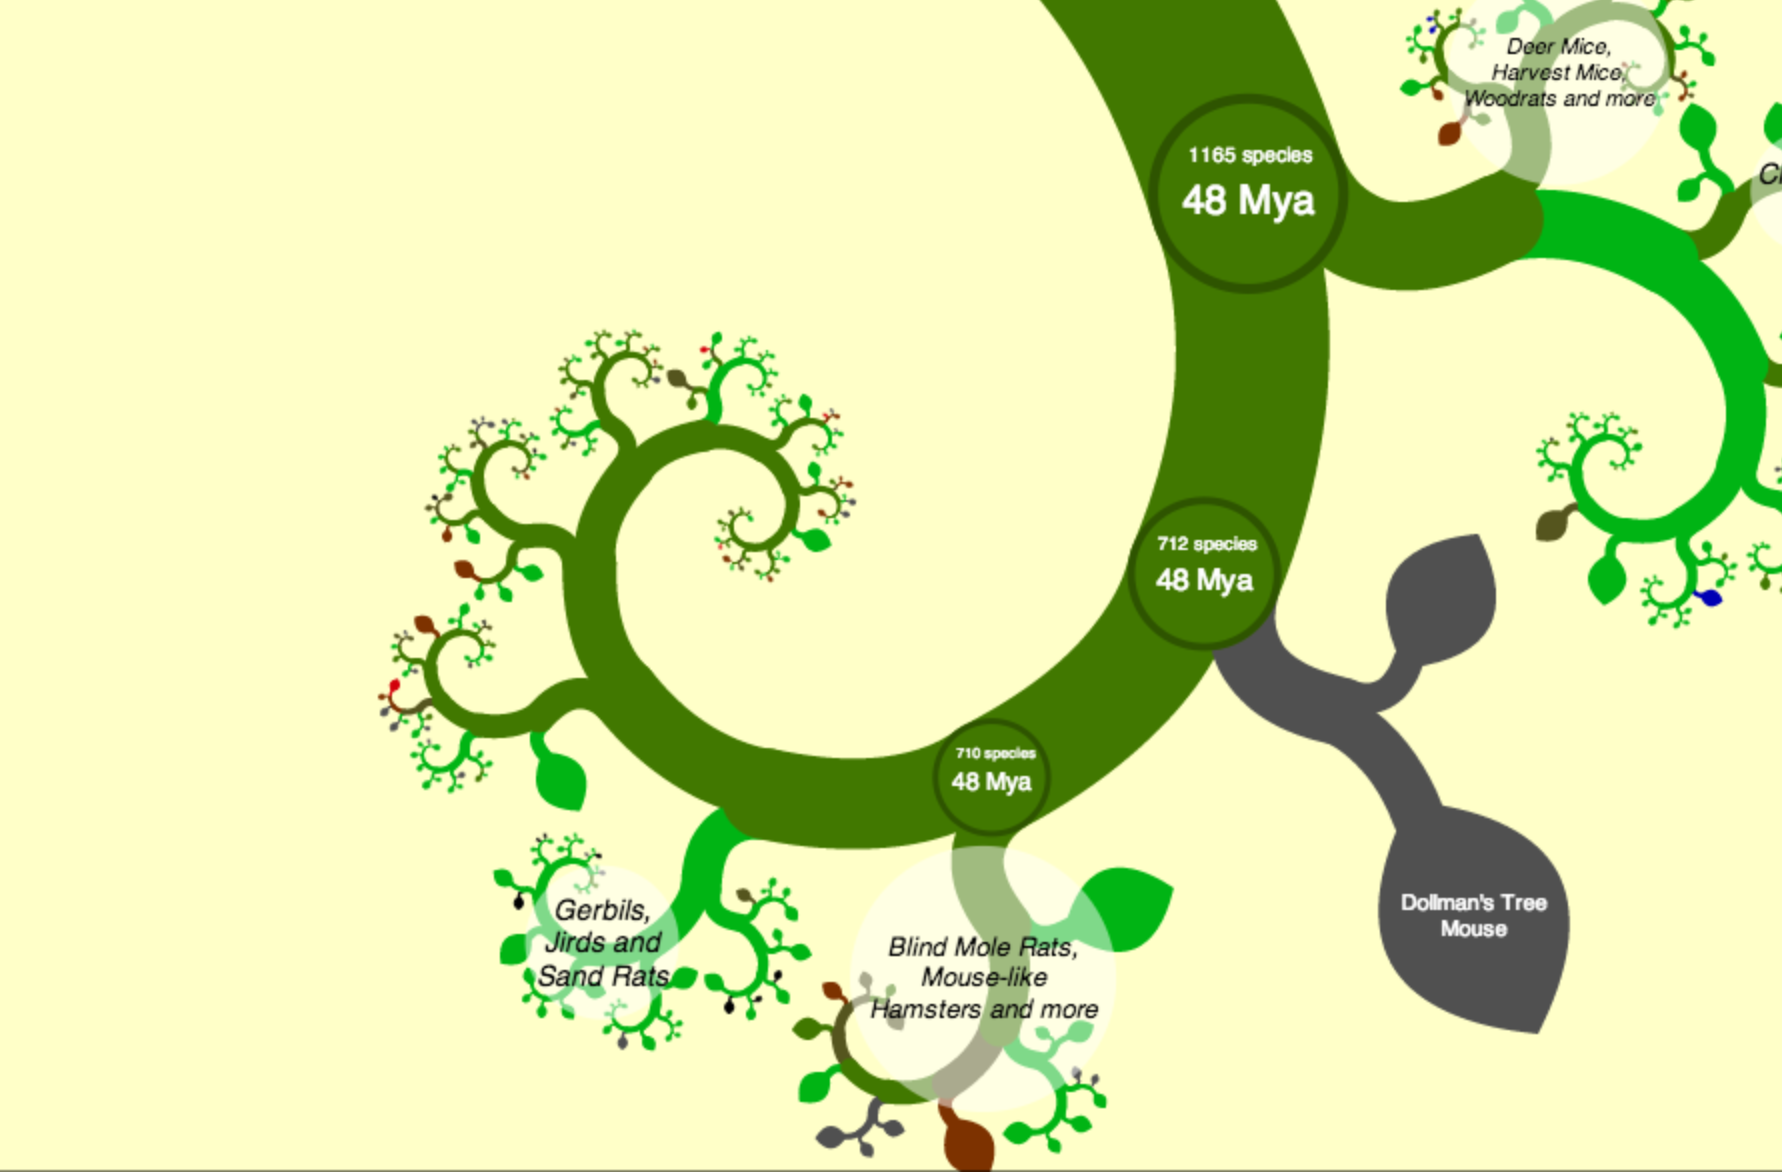
\includegraphics [width=15cm,height=8cm]{MouseLikeRodent}
  \caption{Zoom In the Mouse Like Rodents Branch}
  \label{fig:mouseLikeRodent}
\end{figure}

\section{Software Working Flow}

The software first draw a loading page since that it might take some time for the full tree being loaded and the loading page tells users that the software is still responding. The loading time increases linearly with the size of the species, which could become unacceptable for larger trees. A reasonable solution for shortening loading time can be found in chapter 4: Performance Issue. 

After drawing the loading page, the software starts creating fulltree(Class Name) objects from data. This is followed by initializing some node information, like the age of some nodes, which cannot be got directly from data but has to be calculated from their children nodes. Then pre calculation is called to calculate the bezier curve parameter of each node such that the relative position of each node is known. 

When pre calculation is over, the software will call method to update the view and display the whole tree. From then on, user actions like double click, drag are listened and methods for recalculating the position and scale of node objects will be called. When recalculation is done, the tree will be updated. 

\begin{tikzpicture}[node distance = 6cm, auto]
    % Place nodes
    \node [block] (drawLoading) {Displaying Loading};
    \node [block, below of=drawLoading, node distance = 4cm] (load) {Loading and Pre Calculating};
    \node [block, right of=load, node distance = 5.5cm](update) {Update View};
    \node [block, right of=drawLoading, node distance = 5.5cm] (view) {Displaying Tree};
    \node [block, right of =view, node distance = 5.5cm](operation){Drag or Zoom};
    \node [block, below of=operation, node distance = 4cm](setting){Recalculation or Set Parameters};
    %Draw edges
    \path [line] (drawLoading) -- (load);
    \path [line] (load) -- (update);
    \path [line] (update) -- (view);
    \path [line] (view) -- (operation);
    \path [line] (operation) -- (setting);
    \path [line] (setting) -- (update);
\end{tikzpicture}

\section{Ways to decrease the amount of elements being drawn}

As I mentioned earlier, some nodes become invisible when the user zoom into a bigger scale. The visibility of a node is controlled by a threshold. When the size of a node is smaller than the threshold, then the node should not be drawn, so does all of its children. There are also some other thresholds. Both the node object representing leafs and the node object representing conjunction between branches could show text. The text would appear or disappear, displaying in greater details or in less details. All these are controlled by the relative threshold and the size of these nodes. 

Another way to decrease the amount of elements drawn is to only draw nodes within the screen. Testing  whether the boundary of a node is out of the screen, we can select only the nodes within the screen to draw.

\section{Other functionality}

There are many functionalities in the website software. However, due to limitation on time, I've only implemented two of these functionalities: growth animation and search(Have not yet but expect to). 

Growth animation shows users how a biology tree is developed from the very beginning. The tree grows bigger and shows more and more species as the time increases. This is done by only draw nodes greater or less than a time threshold and change the threshold for every few seconds. 

Search allows users to search a particular key word and move the species where the key word hit into the middle of the screen. If multiple species hit the key word, then user could use next hits to find the next matched species. 

\chapter{OneZoom Android Application Introduction}

In this chapter, I will talk about changes of implementation from the website software to android application. More details concerning how to improve the performance of the software and how to break the memory limitation for larger trees will be discussed in Chapter 4 and Chapter 5.

\section{ }

Instead of using only a fulltree class, this application uses BasicNode as a super class, who takes charge of how to calculate positions of a node, how to get information of a node, and LeafNode, CircleNode as subclasses of BasicNode, who take charge of how to draw themselves. Basically, the tree contains two type of nodes, one is the node with children nodes, the other is the node without any children. The nodes with children will create CircleNode objects, while the other ones will create LeafNode objects. 

In the website software, 


\section{User Operation Listener}

The application now supports three kinds of user interaction: using one finger to drag the tree, double tap to zoom in, using two fingers two zoom in or zoom out. Drag and double tap are detected by inheriting GestureDetector.SimpleOnGestureListener class, while using two finger to zoom is detected by inheriting ScaleGestureDetector.SimpleOnScaleGestureListener class. Then in the subclasses of these listeners, onScroll, onDoubleTap and onScale methods are overrode such that it could call the tree to be recalculated and the view to be updated. 

\begin{lstlisting}
	// event when using two fingers to scale
	@Override
	public boolean onScale(ScaleGestureDetector detector) {
		scaleFactor = detector.getScaleFactor();
		scaleFactor = Math.max(0.5f, Math.min(scaleFactor, 5.0f));
		drawview.zoomin(scaleFactor, detector.getFocusX(), detector.getFocusY());
		return true;
	}
	
	// event when scroll occurs
	@Override
	public boolean onScroll(MotionEvent e1, MotionEvent e2, float distanceX, float distanceY){
		drawview.drag(distanceX, distanceY);
		return true;
	}
	
	// event when double tap occurs    
	@Override
	public boolean onDoubleTap(MotionEvent e) {
		drawview.zoomin(e);
    		return true;
        }

\end{lstlisting}

\chapter{Performance Issue}

Two problems greatly affect the performance of this application. One is over long loading time, the other is slow user interaction response time. Both of the problems are largely influenced by the processing capacity of a mobile phone processor as well as the size of the dataset. 

\section{Loading Time}

Before the phylogenies tree first gets drawn, the application needs to load data from a string and create objects for each logical unit in it, which represents a species or a genre of some species. Then pre calculation which involves all the nodes on the tree gets called in order to calculate the relative position of each node. Both the cost of loading data and the cost of pre calculation is linear. Hence, the loading time of a phylogenies tree is expected to increase linearly with the size of the data. By using a older version of the application, we can test the loading time of different phylogenies trees on a Sumsang Galaxy S3 device. When loading the mammal tree who has 5XXX species, the loading time is XXX seconds, while loading the bird tree who has XXXX species and tetropads tree who has XXXXX species, the loading time increases to XXX seconds and XXX seconds respectively. The increase of loading time with the increase of species can also be observed in the website software. (Figures of the comparison can be seen below). As the ambition of this project is to build a tree of all existing and existed species, which has over million species, the loading time of that tree could be intolerable.

In order to shorten the loading time, several bitmaps of those trees are stored as resources. When a user select one of the tree, the corresponding bitmap would be drawn on canvas. In the meantime, another thread would be created to load data and do pre calculation. The main UI thread and the calculation thread share a flag by which the view object knows whether the pre calculation is done or not. When the pre calculation is on progress and the user drag or zoom on the tree, the view object will use built in method of canvas class to scale or translate the tree. When pre calculation is finished, the calculation thread would send a message to the main UI thread so that it would invalidate itself. 

Essentially, in the previous design, users spend time waiting for the data to be loaded and calculated. In the later design, the tree is drawn using bitmap even before the tree is created. Therefore, from a user perspective, the loading time of any tree could be reduced to unnoticeable. 

\section{User Interaction}

Another factor that could affect user experience is the slow response time for user interaction. When user drag or zoom on the view, the tree gets recalculate to update the position of each node. Only after the recalculation is done, the view gets updated. Hence, when a user operates on a view, he or she must wait for a whole duration of the recalculation. Things get worse when the user drags the view. It would get a set of mouse move messages, hence that the recalculation would be called for equal times at a very short time. For instance, a single finger move from the middle of the screen to the middle right of the screen could generate XX to XX mouse move messages. The recalculation method will be called XX to XX times after that, which could cause great delay in displaying the tree.

    
\begin{tikzpicture}[node distance = 6cm, auto]
    % Place nodes
    \node [block] (view) {View};
    \node [block, right of=view] (operation) {Drag or Zoom};
    \node [block, below of=operation, node distance = 3cm](recalculation) {Recalculation};
    \node [block, left of=recalculation] (update) {Invalidate View};
    %Draw edges
    \path [line] (view) -- (operation);
    \path [line] (operation) -- (recalculation);
    \path [line] (recalculation) -- (update);
    \path [line] (update) -- (view);
\end{tikzpicture}

\subsection{Using thread and message queue to discard extra mouse move message}

In order to faster the response time, the extra mouse move messages should be discarded. Another thread and message queue is used to solve this problem. When a user triggers a set of mouse move actions, a set of recalculation messages will be sent from the main UI thread to the calculation thread. In the calculation thread, when it catches a recalculation message while there are other recalculation messages in the message queue, then the current recalculation message will be discarded. Otherwise, the recalculation method will be called. Hence, when there are several recalculation messages being sent, only the last one will be processed. When the recalculation is over, the calculation thread will send message to invalidate the view.  

    
\begin{tikzpicture}[node distance = 5.5cm, auto]
    % Place nodes
    \node [block] (view) {View};
    \node [block, right of=view] (operation) {Drag or Zoom};
    \node [block, below of=operation, node distance=2.5cm] (looper) {Looper};
    \node [block, below of=looper, node distance = 2.5cm] (handler) {Handler};
    \node [block, right of=looper, node distance = 5.5cm] (catcher) {Catch next message};
    \node [decision, below of=handler, node distance = 4.5cm] (decision) {Is the only recalculation message??};
    \node [block, left of=decision] (recalculation) {Recalculation};
    %Draw edges
    \path [line] (view) -- (operation);
    \path [line] (operation) -- node[red] {Send Message} (looper);
    \path [line] (looper) -- (handler);
    \path [line] (handler) -- (decision);
    \path [line] (decision) -| node[red, near end]{Yes}(catcher);
    \path [line] (catcher) -- (looper);
    \path [line] (decision) -- node[red]{No}(recalculation);
    \path [line] (recalculation) -- node[red]{Update View}(view);
\end{tikzpicture}

\subsection{Using cached bitmap to update view before calculation is done}
 
 Though the number of calculation messages being processed would be reduced to a minimum number, users would still feel a bit delay in refreshing the view since it gets updated after the recalculation is done. Moreover, as only the last recalculation message in the message queue gets processed, the tree will be placed to the position where the last mouse move message was triggered. This could result in inconsistent display. 

This problem is solved by using cached bitmap to update the view. When the application observes a user operation, it will not only send message to another thread, but also update the view. Then in the onDraw method of the view class, it would test whether the recalculation is done. If it is done, it will draw the tree objects, otherwise it will translate or scale the bitmap stored previously to give users a continuous display. When the recalculation is done, it will send message to update the view. From a user perspective, when he or she drag on the view, he or she would get a consistent display. However, if the user zoom in, he or she would get a unclear picture first, since scaling on bitmap is only scaling on pixels. However, a precise picture of the tree would replace the unclear one soon. 

\begin{tikzpicture}[node distance = 4cm, auto]
    % Place nodes
    \node [block] (recalculation) {Recalculation};
    \node [block, below of=recalculation] (view) {View};
    \node [block, right of=view, node distance = 5.5cm] (operation) {Drag or Zoom};
    \node [block, right of=operation, node distance = 5.5cm] (update) {Update View};
    \node [decision, below of=update, node distance = 4cm] (test) {Test whether should use bitmap};
    \node [block, left of=test, node distance = 5.5cm] (bitmap) {Translate and Scale bitmap};
    \node [block, below of=test] (redraw) {Draw Using Node Object};
    \node [block, left of=redraw, node distance = 5.5cm] (store) {Cache New Bitmap};

    %Draw edges
    \path [line] (view) -- (operation);
    \path [line] (operation) |- node[red, near start, right]{Send Message to Another Thread}(recalculation);
    \path [line] (recalculation) -- node[red] {Send Message to Update View} (view);
    \path [line] (operation) -- (update);
    \path [line] (update) -- (test);
    \path [line] (test) -- node[red, near end]{Yes}(redraw);
    \path [line] (redraw) -- (store);
    \path [line] (test) -- node[red]{No}(bitmap);
    \path [line] (store) -| (view);
    \path [line] (bitmap) -| (view);
\end{tikzpicture}

Lastly, there is one more thing need to be fixed. When the processor of a mobile device is switched to handle recalculation message, it could quickly discard all but the last recalculation message and process it. However, while the recalculation is undertook, user could continue operating on the mobile device. For example, the calculation thread may be switched while the user is moving his or her finger on the screen. As a result, when the calculation is done, the position of the tree object is not where the user's finger point to. If the tree gets drawn this time, the user could see the tree gets dragged back. In order to solve this bug, we need to check whether the recalculation is triggered by the nearest user operation. Two counter are created for the check. One is incremented when a recalculation message is generated. The other is incremented when a recalculation message is received in another thread. When two counters are equal, then the last recalculation message is under processed or has been processed. To prevent the view gets redrawn using the node tree while recalculation is undertaking, a boolean variable is set to false when recalculation message is sent and is set to false when recalculation is done. Together with two counters, it could ensure the tree only gets drawn by the tree object when the recalculation has been done and it is corresponding to the last user operation. 

\begin{tikzpicture}[node distance = 4cm, auto]
    % Place nodes
    \node [block] (test) {Test whether should use bitmap};
	\node [decision, right of=test, node distance = 5.5cm](counter){Counter equals};
	\node [decision, right of=counter, node distance = 5.5cm](during){During recalculation};
	\node [block, below of=counter, node distance =3.5cm] (bitmap) {Using bitmap};
	\node [block, below of=bitmap, node distance = 2.5cm] (redrawn) {Using Node Object};
    %Draw edges
     \path [line] (test) -- (counter);
    \path [line] (counter) -- node[red] {Yes} (during);
    \path [line] (counter) -- node[red] {No} (bitmap);
    \path [line] (during) |- node[red, near end] {Yes} (bitmap);
    \path [line] (during)|- node[red, near end] {No} (redrawn);
\end{tikzpicture}




\chapter{Memory Issue}



\chapter{Functionality}


\begin{thebibliography}{123}
\addcontentsline{toc}{chapter}{Bibliography}
\raggedright

\bibitem{bibtex} It is more convinient and faster to use \texttt{bibtex} instead 
of writing your bibliography manually.

\bibitem{jabref}
You can even use a tool like \texttt{jabref} to manage and maintain your 
database of references.

\end{thebibliography}

\end{document}

%%%%%%%%%%%%%%%%%%%%%%%%%%%%%%%%%%%%%%%%%%%%%%%%%%%%%%%%%%%%%%%%%%%%
%
% If you print your dissertation for yourself or as a present for
% family, friends or colleagues you probably should use a different
% layout which does not fulfill the College requirements but which
% can look much better.
%
% For further information and for professional layouting and
% printing services please visit www.PrettyPrinting.net
%
%%%%%%%%%%%%%%%%%%%%%%%%%%%%%%%%%%%%%%%%%%%%%%%%%%%%%%%%%%%%%%%%%%%%